\section{Results}
\label{sec:results}

The results answer the production question directly: with the candidate universe, target surface, and
record budget fixed, which retained weight vector best fits the current \populace{} target surface? All
methods are scored on the full set of 32{,}633 materialized targets, using the penalty-free Populace
objective loss in Equation~\ref{eq:loss_cal}. The run reported here is a matched full-scale probe rather
than a full budget frontier: a normalized $L_0$ penalty selects a sparse support, the same retained count
is used for the post-$L_0$ refit and sparse baselines, and an epoch-matched dense no-$L_0$ calibration
anchors the comparison. Raw absolute-relative-error (ARE) summaries, effective sample size, and max weight
are reported as diagnostics around the headline loss.

\subsection{The full-surface matched probe}

Figure~\ref{fig:objective_frontier} is the headline result. On the current three-year ASEC support file,
the normalized $L_0$ penalty selects 57{,}240 of 337{,}704 candidate households, or 17.0\% of the
candidate universe. The raw gated $L_0$ weights are not the right publication weights: scored after
thresholding, they reach a Populace objective loss of 9.86\%. Removing the gates and refitting ordinary
calibration weights on exactly the selected records lowers that loss to 4.74\%. A dense no-$L_0$
calibration using all 337{,}704 records and the same 1{,}500-epoch optimizer budget reaches 5.07\%. A
random subset of the same size as the $L_0$ support, followed by the same 1{,}500-epoch gradient
reweighting, reaches 7.55\%. A random subset of the dense calibrated weights, scaled back to the dense
total but not refit, reaches 24.24\%.

The practical interpretation is that the $L_0$ selector is doing useful support-selection work, but the
post-selection refit is essential. The selected support gives a lower finite-budget optimizer loss than
the full dense run at 1{,}500 epochs and fits the full target surface much more closely than a random
support of the same size. This should not be read as a claim that the dense feasible set is worse: the
dense no-$L_0$ loss is still declining at the end of the 1{,}500-epoch budget. The defensible claim is that
this $L_0$ support gives a better sparse support and a faster route to low loss under the completed
optimizer budget. The current evidence should still be read as a single fixed-penalty probe, not as proof
that this exact penalty is optimal: the next sweep needs to trace the normalized penalty across multiple
retained counts and concentration settings.

\begin{figure}[H]
    \centering
    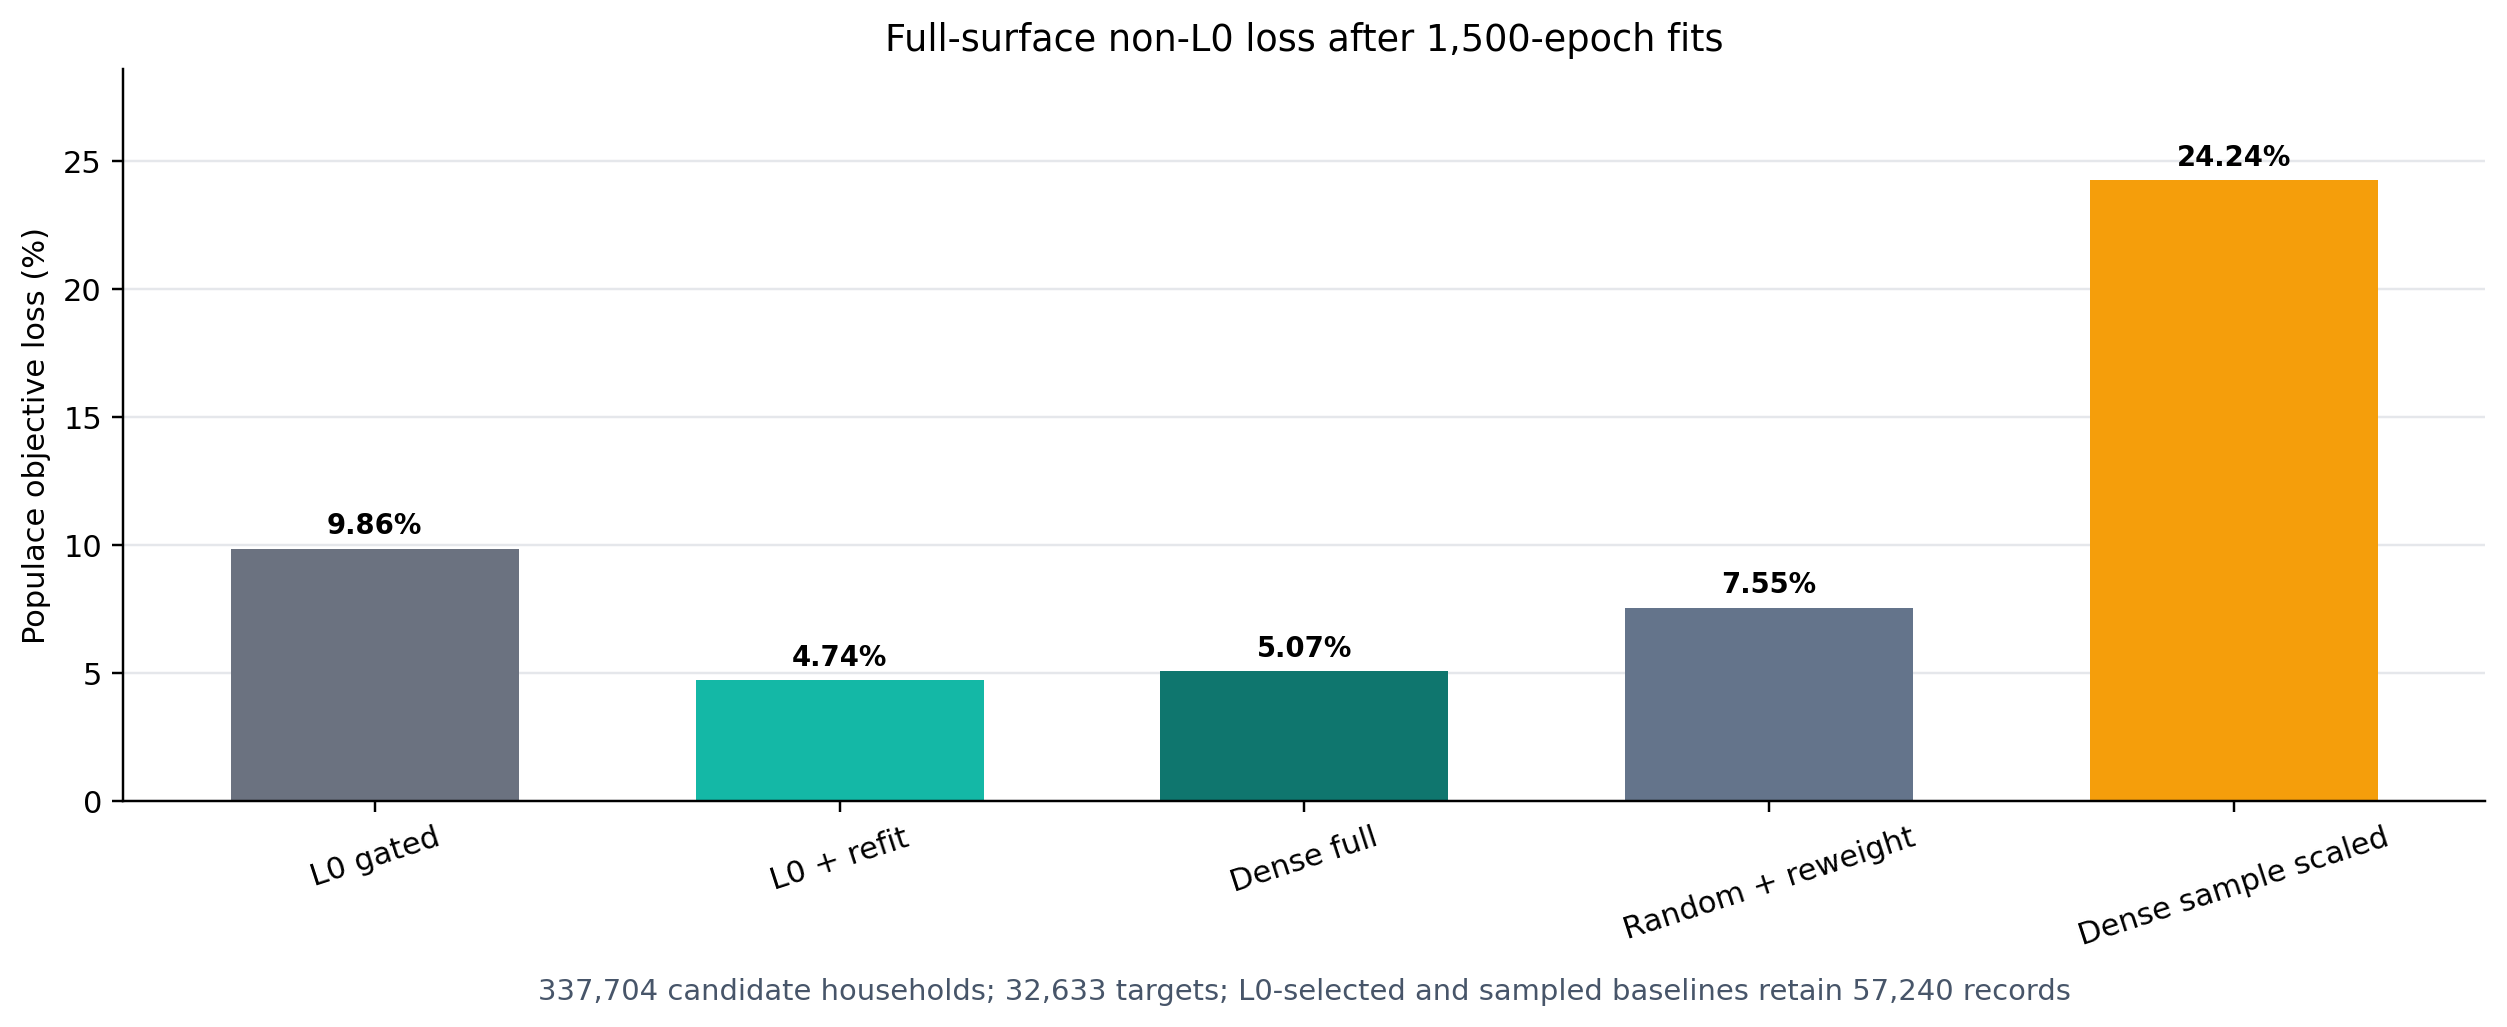
\includegraphics[width=0.96\textwidth]{figures/f0_objective_frontier}
    \caption{Full-surface Populace objective loss in the matched probe. The objective is the capped,
    target-weighted calibration loss in Equation~\ref{eq:loss_cal}, evaluated on each method's final
    retained/sampled weight vector and excluding sparsity or concentration penalties. The $L_0$ run uses a
    normalized penalty share of 0.8, equivalent to raw $\lambda_{L_0}=2.37\times10^{-6}$ for 337{,}704
    candidate households.}
    \label{fig:objective_frontier}
\end{figure}

Table~\ref{tab:sampling_comparison} reports the same comparison with raw ARE and weight diagnostics. The
median ARE gives a different view from the capped objective: dense no-$L_0$ has the lowest median ARE
(0.56\%), while the post-$L_0$ refit is close (0.89\%) and has the lowest capped Populace loss. Random +
reweight has 6.70\% median ARE, raw gated $L_0$ has 11.66\%, and the dense random scaled sample has
55.24\%. The mean ARE remains much larger because a small tail of difficult IRS targets can have very
large relative misses even when the capped Populace loss is low.

\begin{table}[ht]
\centering
{\tablefont
\resizebox{\textwidth}{!}{%
\begin{tabular}{p{0.20\textwidth}rrrrrr}
\toprule
Method & Budget & In-sample median ARE (\%) & Out-of-sample median ARE (\%) & Out-of-sample mean ARE (\%) & ESS & Max weight \\
\midrule
Informed $L_0$ & 10{,}000 & \multicolumn{5}{c}{\tbc[from \texttt{expanded-5seed}]} \\
Random + reweight & 10{,}000 & \multicolumn{5}{c}{\tbc[from \texttt{expanded-5seed}]} \\
Survey-weight (Hansen--Hurwitz) & 10{,}000 & \multicolumn{5}{c}{\tbc[from \texttt{expanded-5seed}]} \\
\bottomrule
\end{tabular}
}
}
\caption{Informed $L_0$ sampling against the two matched-budget baselines at a representative budget (the
$\sim$10{,}000-record anchor of Figure~\ref{fig:budget_frontier}). All methods share the candidate
universe, the target set, and the fixed family-level holdout, and differ only in how records are
selected. ARE is absolute relative error across the scored targets; the median is the headline read and
the mean is reported alongside as tail-sensitive. ESS is the Kish effective sample size, reported as an
output diagnostic because a sampler can fit the targets while concentrating population mass on a few
records. Cells are the cross-seed summary over five seeds.}
\label{tab:sampling_comparison}
\tablenote{The matched record budget and target counts are read from each run's manifest; the
out-of-sample columns score the held-out families. The survey-weight baseline is the unbiased
Hansen--Hurwitz integerisation (probability-proportional-to-size with replacement). Informed $L_0$ runtime
includes the eight-step budget bisection that sets $\lambda_{L_0}$; the baselines are run once at the
matched budget. Runtime and the family macro-average are reported in the run summary.}
\end{table}


Table~\ref{tab:paired_comparison} expresses the comparison on the headline loss scale. Relative to dense
no-$L_0$, the post-$L_0$ refit lowers the completed-run Populace objective by 6.4\%. Relative to random +
reweight, it lowers the objective by 37.2\%. Relative to the raw gated $L_0$ weights, it lowers the
objective by 51.9\%. The comparison isolates the value of the support and the refit: keeping dense weights
on a random retained set and merely scaling them back to total mass performs poorly, so a sparse file still
needs a reweighting step.

\begin{table}[H]
\centering
{\tablefont
\begin{tabular}{lrr}
\toprule
Comparison & Loss difference (pp) & Relative loss change \\
\midrule
Informed $L_0$ + refit vs. dense no-$L_0$ & $-0.33$ & $-6.4\%$ \\
Informed $L_0$ + refit vs. random + reweight & $-2.81$ & $-37.2\%$ \\
Informed $L_0$ + refit vs. raw informed $L_0$ & $-5.12$ & $-51.9\%$ \\
Dense random sample, scaled vs. dense no-$L_0$ & $+19.17$ & $+378.3\%$ \\
\bottomrule
\end{tabular}
}
\caption{Matched loss comparisons for the full-surface probe. Negative values favour the method named
first. Differences are in percentage points of the capped, target-weighted Populace objective loss.}
\label{tab:paired_comparison}
\tablenote{This table is descriptive because the current matched full-scale run uses one seed and one
normalized $L_0$ penalty. Dense no-$L_0$ and the post-selection/refit baselines all use 1{,}500 optimizer
epochs, but dense no-$L_0$ is still slowly declining at the end of that budget.}
\end{table}


\subsection{Size and concentration}
\label{sec:results-controls}

The normalized penalty gives a usable size control in this probe. We parameterize the sparsity price as a
share of the mean calibration loss, $\lambda_{\mathrm{share}}\sum_i\bar{z}_i/n$, rather than as an
unscaled raw coefficient. With $\lambda_{\mathrm{share}}=0.8$, the optimizer retained 57{,}240 records.
This scaling matters operationally: the same raw coefficient has very different meanings when the
candidate universe changes from tens of thousands to hundreds of thousands of records.

The selected support is more concentrated than the full dense calibration but better conditioned than the
matched random sparse baselines. Dense no-$L_0$ has an effective sample size of 5{,}970 and a maximum
weight of 579{,}298. The post-$L_0$ refit has ESS 4{,}726 and maximum weight 913{,}836. Random + reweight
has lower ESS, 2{,}480, and a higher maximum weight, 1{,}163{,}939; the dense random scaled sample is worse
again, with ESS 981 and maximum weight 2{,}176{,}121. The raw gated $L_0$ weights have higher ESS,
6{,}879, but worse target fit, which is why the refit is the publishable sparse variant.

\begin{figure}[H]
    \centering
    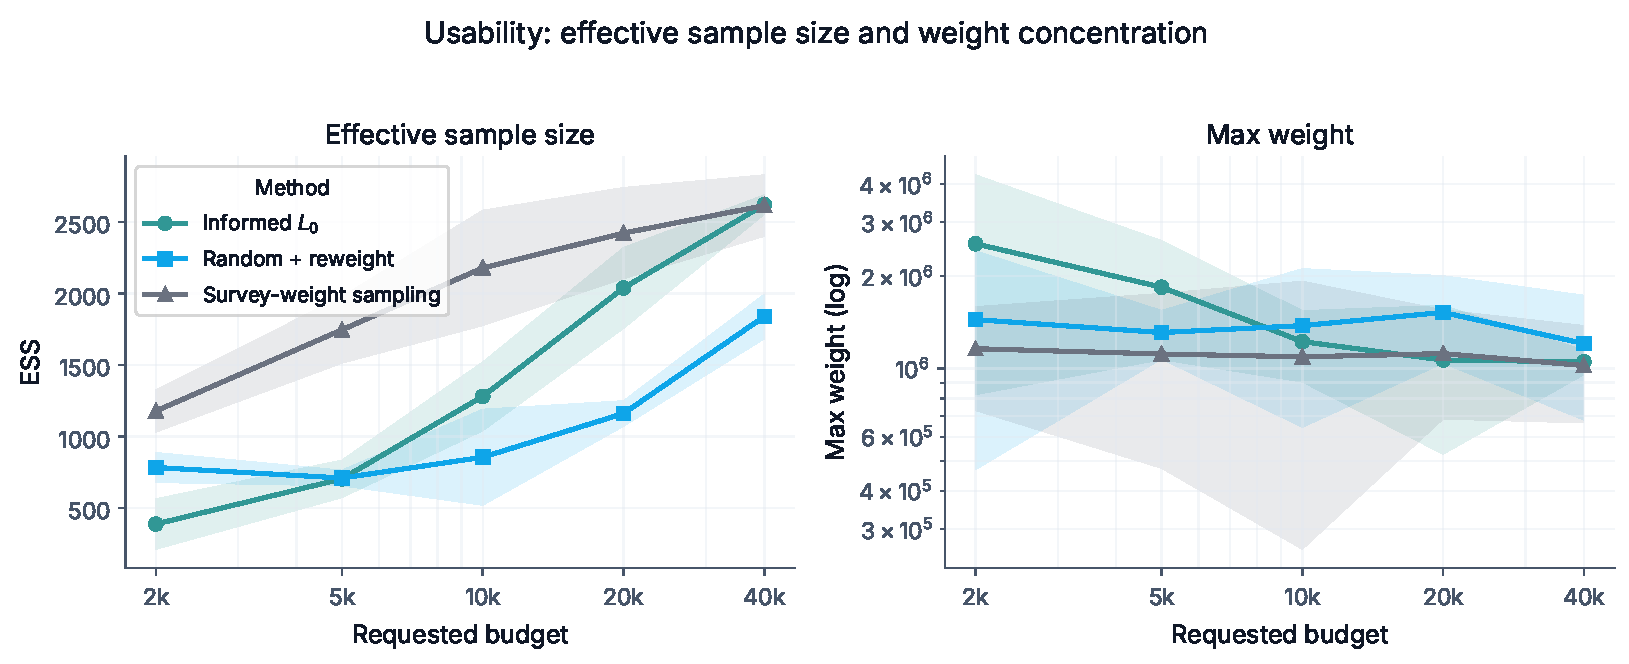
\includegraphics[width=\textwidth]{figures/f2_usability}
    \caption{Weight concentration in the matched full-surface probe. Effective sample size and maximum
    weight are computed on each method's final retained/sampled weight vector. Dense no-$L_0$ retains all
    337{,}704 records; the other sparse rows retain 57{,}240 records.}
    \label{fig:usability}
\end{figure}

\subsection{Accuracy by geography}

Table~\ref{tab:calibration_accuracy} breaks the post-$L_0$ refit diagnostics down by geography. The fit is
strongest at the state level, where median ARE is 0.31\%, followed by national targets at 1.30\% and
district targets at 1.48\%. District targets are the intended stress test for the method: they are the
largest part of the target surface, and they are the reason \populace{} needs to build a large candidate
universe before pruning it.

\begin{table}[H]
\centering
{\tablefont
\begin{tabular}{lrrrr}
\toprule
Geographic level & Targets & Median ARE (\%) & Mean ARE (\%) & Max ARE (\%) \\
\midrule
National & 478 & 1.30 & 20.12 & 557.29 \\
State & 7{,}815 & 0.31 & 86.36 & 122{,}712.20 \\
Congressional district & 24{,}340 & 1.48 & 85.29 & 162{,}495.93 \\
\midrule
\textbf{All scored targets} & 32{,}633 & 0.89 & 84.64 & 162{,}495.93 \\
\bottomrule
\end{tabular}
}
\caption{Calibration accuracy by geographic level for the Informed $L_0$ + refit run at 57{,}240
records, measured as absolute relative error (ARE) across the full target surface. The median reports the
typical target's error; the mean and maximum are tail-sensitive diagnostics.}
\label{tab:calibration_accuracy}
\tablenote{Raw ARE is undefined for 26 IRS SOI national targets where both target and achieved values are
zero; those rows are included in the target count and the Populace loss but omitted from the raw ARE
summary.}
\end{table}


\subsection{Raw-error tails}
\label{sec:results-degenerate}

The Populace objective is the headline score because it is capped and target weighted; raw ARE summaries
are supplemental. In the matched probe, raw ARE is defined for 32{,}607 of the 32{,}633 scored targets.
The remaining 26 rows are IRS SOI national targets with both target and achieved values equal to zero, so
they are omitted from raw relative-error summaries but do not affect the capped loss. Among the defined
rows, the post-$L_0$ refit has a 0.89\% median ARE and an 84.6\% mean ARE. The gap between the median and
the mean is the reason the paper leads with the Populace loss and reports raw ARE only as a diagnostic.

\subsection{Cost}

The matched probe took 39.4 minutes for the $L_0$ selection run. The post-selection refit then added about
9.5 minutes, for a combined 48.9 minutes reported in the artifact. Dense no-$L_0$ took 38.7 minutes for
1{,}500 epochs, random + reweight took 7.3 minutes, and the dense random scaled sample required no extra
optimization beyond the dense fit. The selector is therefore computationally expensive, and the dense run
is still slowly declining at the endpoint. The accuracy gain over dense and random + reweight is large
enough in this probe to justify a broader normalized-penalty sweep, but not enough to skip the next
robustness work: more penalties, longer dense convergence checks, more candidate-support regimes, and
concentration controls.
